%%%%%%%%%%%%%%%%%%%%%%% file template.tex %%%%%%%%%%%%%%%%%%%%%%%%%
%
% This is a general template file for the LaTeX package SVJour3
% for Springer journals.          Springer Heidelberg 2010/09/16
%
% Copy it to a new file with a new name and use it as the basis
% for your article. Delete % signs as needed.
%
% This template includes a few options for different layouts and
% content for various journals. Please consult a previous issue of
% your journal as needed.
%
%%%%%%%%%%%%%%%%%%%%%%%%%%%%%%%%%%%%%%%%%%%%%%%%%%%%%%%%%%%%%%%%%%%
%
% First comes an example EPS file -- just ignore it and
% proceed on the \documentclass line
% your LaTeX will extract the file if required
\begin{filecontents*}{example.eps}
%!PS-Adobe-3.0 EPSF-3.0
%%BoundingBox: 19 19 221 221
%%CreationDate: Mon Sep 29 1997
%%Creator: programmed by hand (JK)
%%EndComments
gsave
newpath
  20 20 moveto
  20 220 lineto
  220 220 lineto
  220 20 lineto
closepath
2 setlinewidth
gsave
  .4 setgray fill
grestore
stroke
grestore
\end{filecontents*}
%
\RequirePackage{fix-cm}
%
\documentclass{svjour3}                     % onecolumn (standard format)
%\documentclass[smallcondensed]{svjour3}     % onecolumn (ditto)
%\documentclass[smallextended]{svjour3}       % onecolumn (second format)
%\documentclass[twocolumn]{svjour3}          % twocolumn
%
\smartqed  % flush right qed marks, e.g. at end of proof
%
\usepackage{graphicx}
\usepackage{amsmath,amssymb}
\usepackage{diffcoeff}
\usepackage{arydshln,mathtools}% http://ctan.org/pkg/{arydshln,leftidx,mathtools}
\usepackage{mathrsfs}
\usepackage{bm}
%\newtheorem{remark}{Remark}

\newcommand{\secref}[1]{\S\ref{#1}}


\DeclareMathOperator{\Tr}{Tr}
\DeclareMathOperator*{\grad}{grad}
\DeclareMathOperator*{\Grad}{Grad}
\DeclareMathOperator*{\Div}{Div}
\renewcommand{\div}{\operatorname{div}}
\DeclareMathOperator*{\Hess}{Hess}

\newcommand{\crmat}[1]{\ensuremath{[#1]_{\times}}}

\def\onedot{$\mathsurround0pt\ldotp$}
\def\cddot{% two dots stacked vertically
	\mathbin{\vcenter{\baselineskip.67ex
			\hbox{\onedot}\hbox{\onedot}}%
}}

% \usepackage{mathptmx}      % use Times fonts if available on your TeX system
%
% insert here the call for the packages your document requires
%\usepackage{latexsym}
% etc.
%
% please place your own definitions here and don't use \def but
% \newcommand{}{}
%
% Insert the name of "your journal" with
\journalname{Multibody System Dynamics}

\makeatletter \renewcommand\d[1]{\ensuremath{%
		\;\mathrm{d}#1\@ifnextchar\d{\!}{}}}
\makeatother

\graphicspath{{./Figures/}}

\begin{document}

\title{Port-Hamiltonian Flexible Multibody Dynamics%\thanks{Grants or other notes
%about the article that should go on the front page should be
%placed here. General acknowledgments should be placed at the end of the article.}
}
\subtitle{}

%\titlerunning{Short form of title}        % if too long for running head

\author{First Author         \and
        Second Author %etc.
}

%\authorrunning{Short form of author list} % if too long for running head

\institute{F. Author \at
              first address \\
              Tel.: +123-45-678910\\
              Fax: +123-45-678910\\
              \email{fauthor@example.com}           %  \\
%             \emph{Present address:} of F. Author  %  if needed
           \and
           S. Author \at
              second address
}

\date{Received: date / Accepted: date}
% The correct dates will be entered by the editor


\maketitle

\begin{abstract}
Insert your abstract here. Include keywords, PACS and mathematical
subject classification numbers as needed.
\keywords{First keyword \and Second keyword \and More}
% \PACS{PACS code1 \and PACS code2 \and more}
% \subclass{MSC code1 \and MSC code2 \and more}
\end{abstract}

\section{Introduction}
\label{intro}
Your text comes here. Separate text sections with

\section{Flexible dynamics}

The coupled ODE-PDE system representing the motion of a single flexible body are here recalled. The model for the classical equations derived using the principle of virtual work can be found in \cite{MB_Daepde}. The small difference with respect to the derivation therein is that the equation for the translation is now written in the body frame. Consider an open connected set $\Omega \in \mathbb{R}^d$, representing a floating flexible body. The dynamics is computed at a generic point $P$, that is not necessarily the center of mass. The velocity of a generic point is the expressed by considering a small flexible displacement superimposed to the rigid motion
\[
v = v_P + \crmat{\omega_P} (x+u_f) + \dot{u}_f,
\]
where $v_P$ is the velocity of point $P$ evaluated in the body reference frame
 The body is assumed to be floating. 

\begin{equation}
\label{eq:rig_tr1}
\begin{split}
&m (\dot{{v}}_P + \crmat{\omega_P}v_P) + \crmat{s_u}^\top \dot{{\omega}}_P  + \int_{\Omega} \rho \ddot{u}_f \d{\Omega} = \\
&\quad - \crmat{\omega_P} \crmat{\omega_P} {s}_u - \int_{\Omega} 2 \rho \crmat{\omega_P} \dot{u}_f \d{\Omega} +  \int_{\Omega} \beta \d{\Omega} + \int_{\partial \Omega} \tau \d{\Gamma} 
\end{split}
\end{equation}

\begin{equation}
\label{eq:rig_rot1}
\begin{split}
\crmat{s_u} (\dot{{v}}_P + \crmat{\omega_P} v_P) + J_u \dot{\omega}_P + \int_{\Omega} \rho \crmat{x+u_f} \ddot{u}_f \d{\Omega} - \crmat{\omega_P} J_u \omega_P = \\ 
- \int_{\Omega} 2\rho \crmat{x+u_f} \crmat{\omega_P} \dot{u}_f \d{\Omega} + \int_{\Omega}\crmat{x+u_f} \beta \d{\Omega} + \int_{\partial \Omega}\crmat{x+u_f} \tau \d{\Gamma} \\
\end{split}
\end{equation}

\begin{equation}
\label{eq:flex1}
\rho (\dot{{v}}_P + \crmat{\omega_P} v_P) + \rho (\crmat{\dot{\omega}_P} + \crmat{\omega_P}\crmat{\omega_P})(x + u_f) + \rho (2 \crmat{\omega_P} \dot{u}_f + \ddot{u}_f) = \Div{\Sigma} + \beta,
\end{equation}
where $m = \int_{\Omega} \rho \d{\Omega}$ is the total mass,  $s_u = \int_{\Omega} \rho (x + u_f) \d{\Omega}$ is the static moment, $J_u= - \int_{\Omega} \rho \crmat{x+u_f}\crmat{x+u_f} \d{\Omega}$ is the inertia matrix. \\
Considering $v_f := \dot{u}_f, \; \dot{v}_f = \ddot{u}_f + \crmat{\omega_P} \dot{u}_f$ and applying the Jacobi identity Eqs. \eqref{eq:rig_tr1}, \eqref{eq:rig_rot1}, \eqref{eq:flex1} can be rewritten equivalently as \\

Rigid translation
\begin{equation}
\label{eq:rig_tr2}
	\begin{split}
	m\dot{{v}}_P + \crmat{s_u}^\top \dot{{\omega}}_P +   \int_{\Omega} \rho \dot{v}_f \d{\Omega}  = \\
	\left[m v_p + \crmat{s_u}^\top \omega_P +\int_{\Omega} \rho v_f \d{\Omega} \right]_\times \omega_P +  \int_{\Omega} \beta \d{\Omega} + \int_{\partial \Omega} \tau \d{\Gamma}, 
	\end{split}
\end{equation}
Rigid rotation
\begin{equation}
\label{eq:rig_rot2}
\begin{split}
\crmat{s_u} \dot{{v}}_P  + J_u \dot{\omega}_P + \int_{\Omega} \rho \crmat{x+u_f} \dot{v}_f \d{\Omega} = \\
\left[\crmat{s_u}^\top \omega_P + \int_{\Omega} \rho {v}_f \d{\Omega} \right]_\times v_P + \left[\crmat{s_u}v_P + J_u \omega_P + \int_{\Omega} \rho \crmat{x+u_f} \dot{v}_f \d{\Omega} \right]_\times \omega_P + 
\\
\int_{\Omega} \left[\rho v_P + \rho \crmat{x+u_f}^\top \, \omega_P + \rho v_f \right]_\times v_f \d{\Omega} + \int_{\Omega}\crmat{x+u_f} \beta \d{\Omega} + \int_{\partial \Omega}\crmat{x+u_f} \tau \d{\Gamma}
\end{split}
\end{equation}
Flexibility PDE
\begin{equation}
\label{eq:flex2}
\begin{split}
\rho \dot{{v}}_P + \rho \crmat{x+u_f}^\top \dot{\omega}_P  + \rho \dot{v}_f = \\
\left[\rho v_P + \crmat{x+u_f}^\top \omega_P + \rho v_f \right]_\times \omega_P + \Div{\Sigma} + \beta,
\end{split}
\end{equation}
Together with the boundary condition
\begin{equation}
\Sigma \cdot n|_\Gamma = \tau|_\Gamma, \quad \text{$n$ is the outward normal.}
\end{equation}

\section{PH flexible dynamics}
\label{sec:pH_fd}
In this section the flexible dynamics of a floating body is written as a coupled system of ODEs and PDEs in pH form. First of only the kinetic and deformation energy are considered for sake of simplicity. Then a generic potential is introduced, so that the generalized coordinates are included in the formulation. 

\subsection{Formulation without generalized coordinates}
Consider the total energy (Hamiltonian), given by the sum of kinetic and deformation energy (linear elasticity):
\begin{equation}
\begin{aligned}
H = H_{\text{kin}} + H_{\text{def}} = \frac{1}{2} \int_{\Omega} \rho ||v_P + \crmat{\omega_P} (x+u_f) + v_f||^2 + \Sigma \cddot \varepsilon  \d{\Omega},
\end{aligned}
\end{equation}
where $\Sigma$ is the Cauchy stress tensor and $\varepsilon$ is the infinitesimal stress tensor. From linear elasticity theory it is well known that $\varepsilon = \Grad(u)$, where $\Grad=~\frac{1}{2} [\nabla + \nabla^\top]$ and $\Sigma = \mathcal{D} \varepsilon$, where $\mathcal{D}$ is the stiffness tensor. The inner product $A \cddot B = \Tr(A B^T)$ is the tensor contraction. \\  
The momenta (usually called energy variables in the pH framework) are then computed by derivation of the Hamiltonian. As the variables belong to finite- and infinite-dimensional spaces the derivative is either a classical gradient either a variational derivative:
\begin{equation}
\label{eq:momenta}
\begin{aligned}
p_t &:= \diffp{H}{v_P} = m v_P + \crmat{s_u}^\top \, \omega_P + \int_{\Omega} \rho v_f \d{\Omega}, \\
p_r &:= \diffp{H}{\omega_P} = \crmat{s_u} v_P + J_u \omega_P + \int_{\Omega} \rho \crmat{x+u_f} v_f \d{\Omega}, \\
p_f &:= \diffd{H}{v_f} = \rho v_P + \rho \crmat{x+u_f}^\top \, \omega_P + \rho v_f, \\
\varepsilon &:= \diffd{H}{\Sigma}
\end{aligned}
\end{equation}
The relation between energy and co-energy variable is then given by
\begin{equation}
\label{eq:mass_op}
\begin{bmatrix}
p_t \\ p_r \\ p_f \\ \varepsilon \\
\end{bmatrix} = 
\underbrace{\begin{bmatrix}
	m & \crmat{s_u}^\top & \mathcal{I}_\rho^{\Omega} & 0 \\
	\crmat{s_u} & J_u & \mathcal{I}_{\rho x}^{\Omega} & 0  \\
	(\mathcal{I}_\rho^{\Omega})^* & (\mathcal{I}_{\rho x}^{\Omega})^* & \rho & 0  \\
	0 & 0 & 0 & {\mathcal{D}}^{-1} \\
	\end{bmatrix}}_{\mathcal{M}: \; \text{Mass operator}}
\begin{bmatrix}
v_P \\ \omega_P  \\ v_f  \\ \Sigma \\
\end{bmatrix},
\end{equation}
where the operators are defined as
\begin{equation*}
\begin{aligned}
\mathcal{I}_\rho^\Omega &:=\int_{\Omega} \rho (\cdot) \d{\Omega}, \\
(\mathcal{I}_\rho^{\Omega})^* &:= \rho, \\
\end{aligned} \qquad
\begin{aligned} 
\mathcal{I}_{\rho x}^{\Omega} &:= \int_\Omega \rho \crmat{x+u_f} (\cdot) \d{\Omega}, \\
(\mathcal{I}_{\rho x}^{\Omega})^* &:= \rho \crmat{x+u_f}^\top. \\
\end{aligned}
\end{equation*}
The superscript $*$ denotes the adjoint operator. The mass operator $\mathcal{M}$ is a self-adjoint, positive operator. \\
If the dependency of $\mathcal{M}$ on the flexible displacement $u_f$ is neglected then Eqs. \eqref{eq:rig_rot2}, \eqref{eq:rig_tr2}, \eqref{eq:flex2} can be recast into port Hamiltonian form in co-energy variables
\begin{equation}
\label{eq:ph_mfd}
\mathcal{M}
\diff{}{t}
\begin{bmatrix}
v_P \\ \omega_P  \\ v_f  \\ \Sigma \\
\end{bmatrix} = 
\underbrace{\begin{bmatrix}
0 & \crmat{p_t} & 0 & 0 \\
\crmat{p_t} & \crmat{p_r} & \mathcal{I}_{p_f}^\Omega & 0 \\
0 & -(\mathcal{I}_{p_f}^\Omega)^* & 0 & \Div \\
0 & 0 & \Grad & 0 \\
\end{bmatrix}}_{\mathcal{J}: \; \text{Interconnection operator}}
\begin{bmatrix}
v_P \\ \omega_P  \\ v_f  \\ \Sigma \\
\end{bmatrix} + 
\underbrace{\begin{bmatrix}
\mathcal{I}^\Omega \\
\mathcal{I}_{x}^\Omega \\
I \\
0 \\
\end{bmatrix}}_{\mathcal{B}_d}
\beta + 
\underbrace{\begin{bmatrix}
\mathcal{I}^\Gamma \\
\mathcal{I}_{x}^\Gamma \\
0 \\
0 \\
\end{bmatrix}}_{\mathcal{B}_r} \tau,
\end{equation}
The operator $\mathcal{I}_{p_f}^\Omega = \int_\Omega \crmat{p_f}(\cdot) \d{\Omega}$ has formal adjoint  given by $(\mathcal{I}_{p_f}^\Omega)^* = - \crmat{p_f}(\cdot)$.\\

 The control operators read
\begin{equation*}
\begin{aligned}
\mathcal{I}^\Omega &:=\int_{\Omega} (\cdot) \d{\Omega}, \\
\mathcal{I}^\Gamma &:= \int_{\partial \Omega} (\cdot) \d{\Gamma}, \\
\end{aligned} \qquad
\begin{aligned} 
\mathcal{I}_{x}^\Omega &:=\int_{\Omega} \crmat{x+u_f} (\cdot) \d{\Omega}, \\
\mathcal{I}_{x}^\Gamma &:=\int_{\partial \Omega} \crmat{x+u_f} (\cdot) \d{\Gamma}. \\
\end{aligned}
\end{equation*}
It is important to highlight that $\Div$ and $\Grad$ are formally skew-adjoint operators, i.e. for homogeneous boundary conditions $\tau= 0$
\begin{align*}
\int_{\Omega} \Sigma \cddot \Grad(v_f) \d{\Omega} &\underbrace{=}_{\text{I.B.P.}} -\int_{\Omega} \Div(\Sigma) \cdot v_f \d{\Omega}, \\
\left\langle \Sigma, \, \Grad(v_f) \right\rangle_{\mathscr{L}^2(\Omega, \mathbb{R}^{d\times d}_{\text{sym}})} &\underbrace{=}_{\text{I.B.P.}} -\left\langle\Div(\Sigma), \, v_f \right\rangle_{\mathscr{L}^2(\Omega, \mathbb{R}^d)}, 
\end{align*}
where $\left\langle ,  \right\rangle_\mathscr{H}$ denote an inner product over the Hilbert space $\mathscr{H}$. \\
$\mathscr{L}^2(\Omega, \mathbb{R}^d), \; \mathscr{L}^2(\Omega, \mathbb{R}^{d\times d}_{\text{sym}})$ are the spaces of square integrable vector-valued or symmetric tensors-valued functions in a geometric domain of dimension $d$. \\
For this reason operator $\mathcal{J}_{}$ is skew-symmetric $\mathcal{J}_{}^* = - \mathcal{J}_{}$.

\begin{remark}
If case of vanishing deformation $u_f \equiv 0$ the Newton-Euler equations on $SE(3)$ are retrieved
\begin{equation}
\begin{bmatrix}
\dot{p}_t \\ \dot{p}_r \\
\end{bmatrix} = 
\begin{bmatrix}
	0 & \crmat{p_t}\\
	\crmat{p_t} & \crmat{p_r} \\
	\end{bmatrix}
\begin{bmatrix}
v_P \\ \omega_P  \\
\end{bmatrix} + 
\begin{bmatrix}
f \\ m \\
\end{bmatrix}.
\end{equation}
This system is again in port Hamiltonian form with total energy equal to the kinetic energy.
\end{remark}
\subsection{Including the generalized coordinates}
For the time being only kinetic and deformation energy were considered. If a generic potential energy contribution has to be considered one must account for the generalized coordinates
\begin{itemize}
	\item $^i r_P$: the position of point $P$ in the inertial frame of reference;
	\item $R$: the orientation matrix that transforms vectors from the body frame to the inertial frame (other attitude parametrization are possible, here the orientation matrix is considered for ease of presentation);
	\item $u_f$ the flexible displacement;
\end{itemize}
In particular following \cite{attitude_ph} the orientation matrix is converted in a vector by concatenating its rows
\begin{equation*}
	R_{\text{v}} = \text{vec}(R^\top) = [R_x \; R_y \; R_z]^\top,
\end{equation*}
where $R_{x}, R_{y}, R_{z}$ are the first, second and third row of matrix $R$. Furthermore the corresponding cross map will be given by
\begin{equation*}
\crmat{R_{\text{v}}} = 
\begin{bmatrix}
\crmat{R_x} \\
\crmat{R_y} \\
\crmat{R_z} \\
\end{bmatrix} \qquad 
\crmat{R_{\text{v}}} : \mathbb{R}^9 \rightarrow \mathbb{R}^{9 \times 3}
\end{equation*}

The total energy now includes a potential energy that depends on the generalized coordinates
\begin{equation*}
H = H_{\text{kin}} + H_{\text{def}} + H_{\text{pot}}
\end{equation*}
The overall port Hamitonian formulation is then an augmented version of system~\eqref{eq:ph_mfd}
\begin{equation}
\label{eq:ph_mfd_all}
\setlength{\dashlinegap}{2pt}
\underbrace{
	{\left[ \begin{array}{c:c}
		I & 0 \\
		\hdashline
		0 & \mathcal{M} \\
		\end{array} \right]}
}_{\mathcal{E}}
\diff{}{t}
\underbrace{\begin{bmatrix}
^i r_P \\ R_{\text{v}} \\ u_f \\\hdashline  v_P \\ \omega_P  \\ v_f  \\ \Sigma \\
\end{bmatrix}}_{e} = 
\underbrace{
	{\left[ \begin{array}{ccc:cccc}
		0 & 0 & 0 &  R & 0 & 0 & 0 \\
		0 & 0 & 0 & 0 & \crmat{R_{\text{v}}} & 0 & 0 \\
		0 & 0 & 0 & 0 & 0 & I & 0 \\ 
		\hdashline 
		-R^\top & 0 & 0 & 0 & \crmat{p_t} & 0 & 0 \\
		0 & -\crmat{R_{\text{v}}}^\top & 0 & \crmat{p_t} & \crmat{p_r} & \mathcal{I}_{p_f}^\Omega & 0 \\
		0 & 0 & -I & 0 & -(\mathcal{I}_{p_f}^\Omega)^* & 0 & \Div \\
		0 & 0 & 0 & 0 & 0 & \Grad & 0 \\
		\end{array} \right]}
	}_{\mathcal{J}}
\underbrace{\begin{bmatrix}
\partial_{r_P}H \\ \partial_{R_\text{v}}H \\ \delta_{u_f} H \\\hdashline  v_P \\ \omega_P  \\ v_f  \\ \Sigma \\
\end{bmatrix}}_{z},
\end{equation} 
where the contribution of external forces and torques has been omitted. For example if the gravity potential energy is considered
\begin{equation*}
	H_{\text{pot}} = \int_{\Omega} \rho g \, ^i r^z \d{\Omega} = \int_{\Omega} \rho g \left[ ^i r_{P, z} +R_z (x + u_f) \right] \d{\Omega},
\end{equation*}
the co-energy variables are easily obtained
\begin{align*}
\partial_{r_P}H &= m g \, ^i \widehat{Z}, \quad \text{$^i \widehat{Z}$ is the inertia frame vertical direction}\\
\partial_{R_\text{v}}H &= [0_{(3, 1)}, \; 0_{(3, 1)}, \; \int_{\Omega} \rho g (x + u_f)^\top \d{\Omega}]^\top \\
\delta_{u_f} H &= \rho g \, R_z^\top
\end{align*}
These correspond to the forcing terms due to gravity. System \eqref{eq:ph_mfd_all} fits into the framework detailed in \cite{mehrmann2019structurepreserving} and extends it as a coupled system of ODEs and PDEs is considered. It can be rewritten compactly as follows
\begin{equation}
\label{eq:MFD_pHDAE}
\begin{aligned}
\mathcal{E}(e) \dot{e} &= \mathcal{J}(e) z + \mathcal{B}_d(e) u_d + \mathcal{B}_r(e) u_\partial, \\
y_d &= \mathcal{B}_d^*(e) z, \\
u_\partial &= \mathcal{B}_{\partial} z =  \Sigma \cdot n|_{\Gamma}, \\
y_\partial &= \mathcal{C}_{\partial} z = \partial_t u_f|_{\Gamma}
\end{aligned}
\end{equation}
where $u_d = \beta, \; u_\partial = \tau$. The gradient of the Hamiltonian  gives $\partial_e H = \mathcal{E}^* z$. Adopting the same nomenclature as in \cite{mehrmann2019structurepreserving}, $e$ contains the state and $z$ contains the effort functions. In this case the operators verify $\mathcal{E} = \mathcal{E}^*, \; \mathcal{J} = -\mathcal{J}^*$. The distributed control operator $\mathcal{B}_d$ is bounded. 

\begin{remark}
For sake of simplicity the linear elastic case $H_{\text{def}}=\int_{\Omega} \Sigma \cddot \varepsilon \d{\Omega}$ has been presented. If more complex behaviors have to be accounted for (e.g. geometric stiffening) more complex expression for the deformation energy can be considered. Furthermore, 3D linear elasticity can be simplified and the geometrical dimension reduced. Beam and plate models are represent by appropriate differential operators that replace the $\Div, \Grad$ appearing in \eqref{eq:MFD_pHDAE} (see \secref{sec:ph_floatbeam}).
\end{remark}

\section{Discretization procedure}
\label{sec:discr}
A finite-element based technique to obtain a finite dimensional pH system is illustrated. This methodology relies on the results explained in \cite{cardoso2019partitioned} and boils down to three simple steps
\begin{enumerate}
	\item The system is put into weak form; 
	\item An integration by parts is applied to highlight the proper boundary control;
	\item A Galerkin method is employed to obtain a finite-dimensional system.
\end{enumerate}

\subsection{Illustration for the Elastodynamics PDE}
To explain the methodology consider the elastodynamics PDE
\begin{equation*}
\rho \diffp[2]{u}{t} - \Div\left(\mathcal{D} \Grad(u)\right) = u_d,
\end{equation*}
where a distributed control $u_d$ (a volumetric force) is considered.
The total energy is simply given by 
\[\displaystyle H = \frac{1}{2} \int_{\Omega} \left\{\rho \left(\diffp{u}{t}\right)^2 + \Sigma \cddot \varepsilon \right\} \d{\Omega}.
\]
To get a pH representation the energy variables have to selected. The corresponding co-energies are then computed taking the variational derivative of the Hamiltonian
\begin{equation}
\begin{aligned}
\text{Energies} \quad  x_1 &= \rho \ \partial_t {u}, \\
\text{Co-energies} \quad e_1 &:= \diffd{H}{x_1} =  \partial_t {u}, \\
\end{aligned} \qquad
\begin{aligned}
\mathbb{X}_2 &= \varepsilon = \Grad(u). \\
\mathbb{E}_2 &:= \diffd{H}{\mathbb{X}_2} = \Sigma.
\end{aligned}
\end{equation}
The port-Hamiltonian representation in co-energy variables becomes
\begin{equation*}
\underbrace{\begin{bmatrix}
\rho & 0 \\ 0 & \mathcal{D}^{-1} \\
\end{bmatrix}}_{\mathcal{M}}
\diffp{}{t}
\begin{bmatrix}
e_1 \\ \mathbb{E}_2 \\
\end{bmatrix} = 
\underbrace{\begin{bmatrix}
0 & \Div \\ \Grad & 0 \\
\end{bmatrix}}_{\mathcal{J}}
\begin{bmatrix}
e_1 \\ \mathbb{E}_2 \\
\end{bmatrix} + 
\underbrace{\begin{bmatrix}
1 \\ 0 \\
\end{bmatrix}}_{\mathcal{B}_d} u_d 
\end{equation*}
The interconnection operator may be decomposed as $\mathcal{J} = \mathcal{J}_{\Div} + \mathcal{J}_{\Grad}$
\begin{equation}
\underbrace{\begin{bmatrix}
	0 & \Div \\ \Grad & 0 \\
	\end{bmatrix}}_{\mathcal{J}} = 
\underbrace{\begin{bmatrix}
	0 & \Div \\ 0  & 0 \\
	\end{bmatrix}}_{\mathcal{J}_{\Div}} + 
\underbrace{\begin{bmatrix}
	0 & 0 \\ \Grad & 0 \\
	\end{bmatrix}}_{\mathcal{J}_{\Grad}}
\end{equation}
Assuming a Neumann boundary conditions (the normal traction $\tau$ is known at the boundary),
this system can be written compactly as a boundary control system
\begin{equation}
\label{eq:eldyn_PDE}
\begin{aligned}
\mathcal{M} \diffp{e}{t} &= \mathcal{J} e + \mathcal{B}_d u_d, \\
y_d &= \mathcal{B}_d^* e, \\
u_\partial &= E_2 \cdot n = \Sigma \cdot n|_{\Gamma}, \\
y_\partial &= e_1 = \partial_t u|_{\Gamma}.
\end{aligned}
\end{equation}
Now the system is put into weak form considering the inner product on space $\mathscr{X} = \mathscr{L}^2(\Omega, \mathbb{R}^d) \times \mathscr{L}^2(\Omega, \mathbb{R}^{d\times d}_{\text{sym}})$. Taking two elements $[a, \mathbb{A}], \; [b, \mathbb{B}] \in \mathscr{X}$ the inner product is computed as
\[
\left\langle [a, \mathbb{A}], \ [b, \mathbb{B}] \right\rangle_{\mathscr{X}} = \int_{\Omega} a \cdot b \d{\Omega} + \int_{\Omega} \mathbb{A} \cddot \mathbb{B} \d{\Omega}.
\]
Considering a test function $w \in \mathscr{X}$ the weak form reads
\begin{equation*}
\left\langle w, \; \mathcal{M} \ \partial_t e \right\rangle_{\mathscr{X}} = \left\langle w, \; \mathcal{J} e \right\rangle_{\mathscr{X}} + \left\langle w, \; \mathcal{B}_d u_d \right\rangle_{\mathscr{X}}
\end{equation*}
The bilinear form $m(w, \partial_t e) = \left\langle w, \; \mathcal{M} \ \partial_t e \right\rangle_{\mathscr{X}}$ is symmetric and coercive. The bilinear form $b_d(w, u_d):=\left\langle w, \; \mathcal{B}_d u_d \right\rangle_{\mathscr{X}}$ takes into account distributed control.\\
Now an integration by parts is applied on $\mathcal{J}_{\Div}$
\begin{equation}
\left\langle w, \; \mathcal{J} e \right\rangle_{\mathscr{X}} = \left\langle w, \; \mathcal{J}_{\Grad} e \right\rangle_{\mathscr{X}} - \left\langle \mathcal{J}_{\Grad} w, \; e \right\rangle_{\mathscr{X}} + \left\langle w, \; u_\partial \right\rangle_{\mathscr{L}^2(\Gamma)}
\end{equation}
The expression $j_{\Grad}(w, e) :=\left\langle w, \; \mathcal{J}_{\Grad} e \right\rangle_{\mathscr{X}} - \left\langle \mathcal{J}_{\Grad} w, \; e \right\rangle_{\mathscr{X}}$ is a skew symmetric bilinear form as it holds $j_{\Grad}(w, e)=-j_{\Grad}(e, w)$. The bilinear form $b_{\partial}(w, u_\partial) := \left\langle w, \; u_\partial \right\rangle_{\mathscr{L}^2(\Gamma)}$ imposes weakly the Neumann condition. System \eqref{eq:eldyn_PDE} is now rewritten in weak form
\begin{equation}
m(w, \partial_t e) = j_{\Grad}(w, e) + b_d(w, u_d) + b_{\partial}(w, u_\partial).
\end{equation}
The output equation is discretized considering test function $w_\partial$ defined over the boundary
\begin{equation}
\left\langle w_\partial, \; y_\partial \right\rangle_{\mathscr{X}} = \left\langle w_\partial, \; e_1 \right\rangle_{\mathscr{X}}.
\end{equation}
If a Galerkin method is applied then corresponding test and trial functions are discretized using the same basis
\begin{equation*}
\begin{aligned}
w_1 = \bm{\phi}_1^\top \bm{v}_1, \\
e_1 = \bm{\phi}_1^\top \bm{e}_1, 
\end{aligned} \qquad
\begin{aligned}
\mathbb{W}_2 = \bm{\phi}_2^\top \bm{w}_2, \\
\mathbb{E}_2 = \bm{\phi}_2^\top \bm{e}_2. 
\end{aligned}
\end{equation*}
A finite dimensional pH system is readily obtained
\begin{equation}
\begin{aligned}
{M} \dot{\bm{e}} &= J \bm{e} + {B}_d \bm{u}_d + {B}_\partial \bm{u}_\partial, \\
\bm{y}_d &:= {M}_d \widetilde{\bm{y}}_d = {B}_d^\top \bm{e},  \\
\bm{y}_\partial &:= {M}_\partial \widetilde{\bm{y}}_\partial = {B}_\partial^\top \bm{e}.
\end{aligned}
\end{equation}
Vectors $\widetilde{\bm{y}}_d, \widetilde{\bm{y}}_\partial$ correspond to the output degrees of freedom. The outputs $\bm{y}_d, \bm{y}_\partial$ have been defined incorporating the mass matrix in order get the discrete power balance $\dot{H}_d = \bm{u}_\partial^\top \bm{y}_\partial + \bm{u}_d^\top \bm{y}_d$.

\begin{remark}
Stable mixed finite elements for the elastodynamics problem are detailed in \cite{ArnoldElasDyn}. However the formulation therein is based on a weak form obtained by integration by parts of the $\mathcal{J}_{\Grad}$ operator. The mixed finite element method for such a problem are then stable in the sense of Brezzi thanks to the properties of $L^2 / H^{\Div}$ finite element spaces.
\end{remark}

\subsection{Discretized rigid-flexible Hamiltonian dynamics}

The same methodology is applied to system \eqref{eq:MFD_pHDAE}. If corresponding test functions $w$, state $e$ and the effort functions $z$ are discretized using the same bases
\[ w = \bm{\phi}^\top \bm{w}, \quad e = \bm{\phi}^\top \bm{e}, \quad z = \bm{\phi}^\top \bm{z},
\]
then a finite-dimensional pHDAE system is obtained (after integration by parts of the $\mathcal{J}_{\Div}$ operator as )
\begin{equation}
	\begin{aligned}
	{E}(\bm{e}) \dot{\bm{e}} &= {J(\bm{e}) z} + {B}_d(\bm{e}) \bm{u}_d + {B}_\partial(\bm{e}) \bm{u}_\partial, \\
	\bm{y}_d &:= {M}_d \widetilde{\bm{y}}_d = {B}_d^\top \bm{e},  \\
	\bm{y}_\partial &:= {M}_\partial \widetilde{\bm{y}}_\partial = {B}_\partial^\top \bm{e}.
	\end{aligned}
\end{equation}
The computation of vector $\bm{z}$ is based on the gradient of the discrete Hamiltonian:
\[
\diffp{H_d}{\bm{e}} = {E}^\top \bm{z}, \qquad H_d = H_{d, \text{kin}}+H_{d, \text{def}}+H_{d, \text{pot}},
\]
For the deformation and kinetic energy it is straightforward to find the between the state and effort functions as those energy are quadratic in the state variable:
\begin{equation}
H_{d, \text{kin}} + H_{d, \text{def}} = \frac{1}{2} \bm{e}_{\text{kd}}^\top \, {M}_{\text{kd}} \, \bm{e}_{\text{kd}} \longrightarrow \bm{z}_{\text{kd}} = \bm{e}_{\text{kd}},
\end{equation}
where $\bm{e}_{\text{kd}} = [\bm{v}_P; \, \bm{\omega}_P; \, \bm{v}_f; \bm{\Sigma}]$ and ${M}_{\text{kd}}$ is the discretization of the mass operator $\mathcal{M}$ given in Eq \eqref{eq:mass_op}. 
The only term that requires additional care is the potential energy and particularly the variational derivative of the Hamiltonian with respect to the deformation displacement $z_{u}=\delta_{u_f} H$.  Consider the continuous power balance associate to
\[
\dot{H} = \int_{\Omega} \diffp{u_f}{t} \cdot z_{u} \d{\Omega} = \int_{\Omega} \diffp{u_f}{t} \cdot \diffd{H}{u_f} \d{\Omega}
\]
The deformation velocity and its corresponding effort variable are discretized using the same basis, i.e. $u_f = \bm{\phi}_u^\top \bm{u}_f, \; z_u = \bm{\phi}_u^\top \bm{z}_u$. The discrete Hamiltonian rate assumes two equivalent expressions
\begin{equation*}
\dot{H}_d(\bm{u}_f) = 
\begin{cases}
\dot{\bm{u}}_f^\top {M}_u \; \bm{z}_u, \\
\displaystyle \dot{\bm{u}}_f^\top \diffp{H_d}{\bm{u}_f},
\end{cases}
\end{equation*}
where ${M}_u=\int_{\Omega} \bm{\phi}_u \, \bm{\phi}_u^\top \d{\Omega}$. To preserve the power balance at a discrete level it must hold $ \bm{z}_u = {M}_u^{-1} \diffp{H_d}{\bm{u}_f}$. \\

\begin{remark}\label{rmk:def_P}
So for a uniform Neumann boundary condition has been considered. Indeed, as an unconstrained flexible displacement also produces rigid body motion, it is necessary to constrain the flexible deformation in order to have a non singular mass matrix. If $P$ belongs to the boundary then
a natural choice is to assume zero deformation at point $P$. This is equivalent, in the case of a 1D structure, to a cantilever condition. 
\end{remark}

\subsection{Application to thin planar beams}
\label{sec:ph_floatbeam}

\begin{figure}[t]
	\centering
	\includegraphics[width=0.55\textwidth]{beam.eps} 
	\caption{Floating beam. The rigid motion is located at the initial point P}
	\label{fig:beam}
\end{figure}


If a thin planar flexible beams is considered as mechanical model. $P$ is placed at the origin of the local frame, while $C$ is the ending point of the beam (see Fig. \ref{fig:beam}). The beam has length $L$, Young modulus $E$, density $\rho$, cross section $A$ and second moment of area $I$. The model in strong form for a flexible beam (omitting the partition associated to the generalized coordinate and neglecting the dependence of the mass operator with respect to the deformation) is then written compactly as 
\begin{equation}
\label{eq:EB_str_phdae}
\begin{aligned}
\mathcal{M} \dot{e} &= \mathcal{J}(e) e + \mathcal{B}_r u_\partial, \\
u_\partial &= \mathcal{B}_{\partial} e, \\
y_\partial &= \mathcal{C}_{\partial} e.
\end{aligned}
\end{equation}
Furthermore, the deformation at point $P$ is assumed to be null (see Remark \ref{rmk:def_P}), i.e. $v_f^x(P) = v_f^y(P) = 0$. The state and boundary vectors are expressed as
\begin{align*}
e &= [v_P^x, \; v_P^y, \; \omega_P^z, \; v_f^x, \; v_f^y, \; n_x, \; m_{xx}]^\top, \\
u_\partial &=  [F_{P}^x, \; F_{P}^y, \; T_{P}^z, \; F_{C}^x, \; F_{C}^y, \; T_{C}^z]^\top, \\
y_\partial &=  [v_{P}^x, \; v_{P}^y, \; \omega_{P}^z, \; v_{C}^x, \; v_{C}^y, \; \omega_{C}^z]^\top.
\end{align*}
The state contains the linear and angular velocity $v_P^x, \; v_P^y, \; \omega_P^z$ at point $P$, the deformation velocity $ v_f^x, \; v_f^y$ and the traction and bending stress $n_x, \; m_{xx}$. The boundary input contains the forces and torques acting at the extremities of the beam, while the boundary output contains the velocities at the extremities of the beam.
The cross product are then adapted to the planar case. The mass operator then reads
\begin{equation}
\label{eq:EB_M}
\mathcal{M} = 
\begin{bmatrix}
m & 0 & 0 & \mathcal{I}_\rho^L & 0 & 0 & 0 \\
0 & m & s^x & 0 & \mathcal{I}_\rho^L & 0 & 0 \\
0 & s^x & J^{zz} & 0 & \mathcal{I}_{\rho x}^{L} & 0 & 0 \\
(\mathcal{I}_\rho^{L})^* & 0 & 0 & \rho A & 0 & 0 & 0  \\
0 & (\mathcal{I}_\rho^{L})^* & (\mathcal{I}_{\rho x}^{L})^* & 0 & \rho A & 0 & 0  \\
0 & 0 & 0 & 0 & 0 & {EA}^{-1} & 0 \\
0 & 0 & 0 & 0 & 0 & 0 & {EI}^{-1} \\
\end{bmatrix},
\end{equation}
where  $s^x = \int_{0}^{L} \rho A x \d{x}$ is the static moment, $J^{zz} = \int_{0}^{L} \rho A x^2 \d{x}$ is the moment of inertia, $\mathcal{I}_\rho^L := \int_{0}^L \rho A (\cdot) \d{x}, \; \mathcal{I}_{\rho x}^L := \int_{0}^L \rho A x (\cdot) \d{x}$. The interconnection operator 
\begin{equation}
\label{eq:EB_J}
\mathcal{J}(e) = 
\begin{bmatrix}
0 & 0 & +p_t^y      & 0 & 0 & 0 & 0 \\
0 & 0 & -p_t^x     & 0 & 0 & 0 & 0 \\
-p_t^y & +p_t^x & 0 & -\mathcal{I}_{p_f^y}^{L} & +\mathcal{I}_{p_f^x}^{L} & 0 & 0 \\
0 & 0 & +(\mathcal{I}_{p_f^y}^{L})^* & 0 & 0 & \partial_x & 0  \\
0 & 0 & -(\mathcal{I}_{p_f^x}^{L})^* & 0 & 0 & 0 & -\partial_{xx} \\
0 & 0 & 0 & \partial_{x} & 0 & 0 & 0 \\
0 & 0 & 0 & 0 & \partial_{xx} & 0 & 0 \\
\end{bmatrix}
\end{equation}
where $p_t^x, p_t^y$ are the canonical momenta components, $\mathcal{I}_{p_f^x}^{L} := \int_{0}^{L} p_f^x (\cdot) \d{x}$ and $\mathcal{I}_{p_f^y}^{L} := \int_{0}^{L} p_f^y (\cdot) \d{x}$. And finally the control operator
\begin{equation}
\mathcal{B}_r = \begin{bmatrix}
I_{3\times 3} & \tau_{CP}^\top \\
0_{4\times 3} & 0_{4\times 3} \\
\end{bmatrix} \qquad \text{with} \quad
\tau_{CP} = \begin{bmatrix}
1 & 0 & 0 \\
0 & 1 & L \\
0 & 0 & 1 \\
\end{bmatrix},
\end{equation}

The discretization procedure detailed in \secref{sec:discr} is easily extended to this case considering that the operator to be integrated by parts here is 
\[
\mathcal{J}_{\Div} = \begin{bmatrix}
\partial_x & 0 \\
0 & -\partial_{xx} \\
\end{bmatrix}
\]
The first line and second line are integrated by parts once and twice respectively, so that the boundary forces and momenta are naturally included in the discretized system as inputs. The finite-dimensional system then reads
\begin{equation}
\begin{aligned}
{M} \dot{\bm{e}} &= J(\bm{e}) \bm{e} + {B}_\partial \bm{u}_\partial, \\
\bm{y}_\partial &= {B}_\partial^\top \bm{e}.
\end{aligned}
\end{equation}

This model describes the motion of a flexible floating beam that undergoes small deformations. 

\section{Multibody systems in pH form}
In Sections \secref{sec:pH_fd}, \secref{sec:discr} the pH formulation of a single flexible floating body in infinite- and finite-dimensional form were presented. The construction of a multibody system is accomplished by exploiting the modularity of the port-Hamiltonian framework. Each element of the system is interconnected to the others by means of classical pH interconnections.

\subsection{Interconnections of pHDAE systems}
Consider two pHDAE systems
\begin{equation}
\begin{cases}
E_i \dot{\bm{x}}_i = {J}_i \displaystyle\diffp{H_i}{\bm{x}_i} + {B}_i^{\text{int}} \bm{u}_i^{\text{int}} + {B}_i^{\text{ext}} \bm{u}_i^{\text{ext}}  \vspace{2mm} \\
\bm{y}_i = {B}_i^T  \displaystyle\diffp{H_i}{\bm{x}_i}
\end{cases} \qquad \forall i = 1, 2.
\end{equation}
The interconnection uses the internal control $\bm{u}_i^{\text{int}}$. An interconnection is said to be power preserving if and only if the following holds:
\begin{equation} \label{eq:int_balance}
\langle \bm{u}_1^{\text{int}}, \; \bm{y}_1^{\text{int}} \rangle + \langle \bm{u}_2^{\text{int}}, \; \bm{y}_2^{\text{int}} \rangle = 0.
\end{equation}

The power going out from one system flows in the other in a lossless manner. Two main interconnections of this kind are of interest when coupling system: the gyrator and transformer interconnection.

\paragraph{Gyrator interconnection}
The gyrator interconnection reads
\begin{equation*}
\bm{u}_1^{\text{int}} = -{C} \bm{y}_2^{\text{int}}, \qquad
\bm{u}_2^{\text{int}} = {C}^\top \bm{y}_1^{\text{int}}.
\end{equation*}
This interconnection verifies \eqref{eq:int_balance}. It is easy to verify that from this interconnection, it is obtained
\begin{align*}
\begin{bmatrix}
E_1 & 0 \\ 0 & E_2 \\
\end{bmatrix}
\begin{bmatrix}
\dot{\bm{x}}_1 \\ \dot{\bm{x}}_2 \\
\end{bmatrix} &= 
\begin{bmatrix}
{J}_1 & -{B}_1^{\text{int}} {C} {B}_2^{\text{int} \top} \\ 
{B}_2^{\text{int}} {C} {B}_1^{\text{int} \top}  & {J}_2 \\
\end{bmatrix}
\begin{bmatrix}
\partial_{\bm{x}_1}{H} \\ 
\partial_{\bm{x}_2}{H} \\
\end{bmatrix}+ 
\begin{bmatrix}
{B}_1^{\text{ext}} & 0 \\ 0 & {B}_2^{\text{ext}} \\
\end{bmatrix} 
\begin{bmatrix}
\bm{u}_1^{\text{ext}} \\ \bm{u}_2^{\text{ext}} \\
\end{bmatrix}  \\
\begin{bmatrix}
\bm{y}_1^{\text{ext}} \\ \bm{y}_2^{\text{ext}} \\
\end{bmatrix}  &= \begin{bmatrix}
B_1^{\text{ext} \top} & 0 \\
0 & B_2^{\text{ext} \top} \\
\end{bmatrix} \begin{bmatrix}
\partial_{x_1}{H} \\ 
\partial_{x_2}{H} \\
\end{bmatrix},
\end{align*}
with $H(x_1, x_2) = H_1(x_1) + H_2(x_2)$.

\paragraph{Transformer interconnection}
The transformer interconnection reads
\begin{equation*}
\bm{u}_1^{\text{int}} = -{C} \bm{u}_2^{\text{int}}, \qquad
\bm{y}_2^{\text{int}} = {C}^\top \bm{y}_1^{\text{int}}.
\end{equation*}
Again, this interconnection verifies \eqref{eq:int_balance}. After the interconnection the final system is differential algebraic:
\begin{align*}
\begin{bmatrix}
E_1 & 0 & 0 \\ 
0 & E_1 & 0 \\
0 & 0 & 0 \\
\end{bmatrix}
\begin{bmatrix}
\dot{\bm{x}}_1 \\ \dot{\bm{x}}_2 \\ \dot{\bm{\lambda}} \\
\end{bmatrix} &= 
\begin{bmatrix}
J_1 & 0 & -B_1^{\text{int}} C \\ 
0 & J_2 & B_2^{\text{int}} \\
C^\top B_1^{\text{int} \top} & - B_2^{\text{int} \top} & 0 \\
\end{bmatrix}
\begin{bmatrix}
\partial_{\bm{x}_1}{H} \\ 
\partial_{\bm{x}_2}{H} \\
\bm{\lambda} \\
\end{bmatrix}+ 
\begin{bmatrix}
B_1^{\text{ext}} & 0 \\ 0 & B_2^{\text{ext}} \\ 0 & 0 \\
\end{bmatrix} 
\begin{bmatrix}
\bm{u}_1^{\text{ext}} \\ 
\bm{u}_2^{\text{ext}} \\
\end{bmatrix} \\
\begin{bmatrix}
\bm{y}_1^{\text{ext}} \\ \bm{y}_2^{\text{ext}} \\
\end{bmatrix}  &= \begin{bmatrix}
B_1^{\text{ext} \top} & 0 & 0 \\
0 & B_2^{\text{ext} \top} & 0 \\
\end{bmatrix} \begin{bmatrix}
\partial_{\bm{x}_1}{H} \\ 
\partial_{\bm{x}_2}{H} \\
\bm{\lambda} \\
\end{bmatrix}.
\end{align*}
A transformer interconnection is indeed equivalent to a gyrator interconnection of pHDAE systems.
It is sufficient to interchange the role of output and input of the second system $\bm{u}_2^{\text{int}} \leftrightarrow \bm{y}_2^{\text{int}}$. The output than plays the role of a Lagrange multiplier. 


\subsection{Application to multibody systems of beams}
Once a discretized system is obtained by application of a transformer interconnection lossless joints can be introduced. The simplest example is an hinged link between two beams. In this case the internal variables are
\begin{equation*}
\begin{aligned}
\bm{u}_1^{\text{int}} &= [F^x_{C_1}, \, F^y_{C_1}]^\top := \bm{F}_{C_1}, \\
\bm{u}_2^{\text{int}} &= [F^x_{P_2}, \, F^y_{P_2}]^\top := \bm{F}_{P_2},
\end{aligned} \qquad
\begin{aligned}
\bm{y}_1^{\text{int}} &= [v^x_{C_1}, \, v^y_{C_1}]^\top := \bm{v}_{C_1}, \\
\bm{y}_2^{\text{int}} &= [v^x_{P_2}, \, v^y_{P_2}]^\top := \bm{v}_{P_2}.
\end{aligned}
\end{equation*}
The interconnection matrix is the relative rotation matrix between the two local frames
\begin{equation}
R(\theta) = \begin{bmatrix}
\cos(\theta) & - \sin(\theta) \\
\sin(\theta) & \cos(\theta) \\
\end{bmatrix}, \qquad 
\begin{aligned}
\theta(t) &= \theta(0) + \int_{0}^t (\omega^z_{P_2} - \omega^z_{P_1}) \d{\tau}.
\end{aligned}
\end{equation}

\begin{figure}[t]
	\centering
	\includegraphics[width=0.45\textwidth]{beam_int.eps} 
	\includegraphics[width=0.45\textwidth]{block_hinged_beam.eps} 
	\caption{Two beams interconnected by an hinge }
	\label{fig:beam_int}
\end{figure}

The transformer interconnection
\begin{equation*}
\bm{F}_{C_1} = -R(\theta) \bm{F}_{P_2}, \qquad
\bm{v}_{P_2} = R(\theta)^\top \bm{v}_{C_1}.
\end{equation*}
imposes the constraints on a velocity level and gives rise to an index 2 pHDAE
\begin{align*}
\begin{bmatrix}
E_1 & 0 & 0 \\ 
0 & E_1 & 0 \\
0 & 0 & 0 \\
\end{bmatrix}
\begin{bmatrix}
\dot{\bm{e}}_1 \\ \dot{\bm{e}}_2 \\ \dot{\bm{\lambda}} \\
\end{bmatrix} &= 
\begin{bmatrix}
J_1(\bm{e}_1) & 0 & -B_1^{\text{int}} R(\theta) \\ 
0 & J_2(\bm{e}_2) & B_2^{\text{int}} \\
R(\theta)^\top B_1^{\text{int} \top} & - B_2^{\text{int} \top} & 0 \\
\end{bmatrix}
\begin{bmatrix}
\bm{e}_1  \\ 
\bm{e}_2  \\ 
\bm{\lambda} \\
\end{bmatrix}+ 
\begin{bmatrix}
B_{\partial 1}^{\text{ext}} & 0 \\ 0 & B_{\partial 2}^{\text{ext}} \\ 0 & 0 \\
\end{bmatrix} 
\begin{bmatrix}
\bm{u}_1^{\text{ext}} \\ 
\bm{u}_2^{\text{ext}} \\
\end{bmatrix} \\
\begin{bmatrix}
\bm{y}_1^{\text{ext}} \\ \bm{y}_2^{\text{ext}} \\
\end{bmatrix}  &= \begin{bmatrix}
B_{\partial 1}^{\text{ext} \top} & 0 & 0 \\
0 & B_{\partial 2}^{\text{ext} \top} & 0 \\
\end{bmatrix} \begin{bmatrix}
\bm{e}_1  \\ 
\bm{e}_2  \\ 
\bm{\lambda} \\
\end{bmatrix}.
\end{align*}




% For tables use
\begin{table}
% table caption is above the table
\caption{Please write your table caption here}
\label{tab:1}       % Give a unique label
% For LaTeX tables use
\begin{tabular}{lll}
\hline\noalign{\smallskip}
first & second & third  \\
\noalign{\smallskip}\hline\noalign{\smallskip}
number & number & number \\
number & number & number \\
\noalign{\smallskip}\hline
\end{tabular}
\end{table}


%\begin{acknowledgements}
%If you'd like to thank anyone, place your comments here
%and remove the percent signs.
%\end{acknowledgements}

% BibTeX users please use one of
%\bibliographystyle{spbasic}      % basic style, author-year citations
%\bibliographystyle{spmpsci}      % mathematics and physical sciences
%\bibliographystyle{spphys}       % APS-like style for physics
%\bibliography{}   % name your BibTeX data base
\bibliographystyle{unsrt}
\bibliography{multibody} 

% Non-BibTeX users please use

\end{document}
% end of file template.tex

